% Kestrel slides for the mentor review (Week 16). Build: cd paper/slides && latexmk -pdf kestrel_slides.tex
% Same rule as the paper: every result number is a \kv{key} from ../generated/numbers.tex, written by
% experiments/analysis/paper_assets.py from the committed logs; an unknown key prints as ??key??.
% What to say on each slide: speaker_notes.md next to this file.
\documentclass[aspectratio=169,11pt,xcolor=table]{beamer}
\usepackage[T1]{fontenc}
\usepackage{lmodern}
\usepackage{booktabs}
\usepackage{tikz}
\usetikzlibrary{arrows.meta,calc}

\DeclareRobustCommand{\kv}[1]{\ifcsname kv@#1\endcsname\csname kv@#1\endcsname\else\textbf{??#1??}\fi}
% Generated by experiments/analysis/paper_assets.py from the committed logs.
\makeatletter
\expandafter\def\csname kv@delta\endcsname{\ensuremath{0.0263}}
\expandafter\def\csname kv@clinc.n\endcsname{\ensuremath{5500}}
\expandafter\def\csname kv@clinc.timed\endcsname{\ensuremath{1100}}
\expandafter\def\csname kv@clinc.r0.acc\endcsname{\ensuremath{0.827}}
\expandafter\def\csname kv@clinc.r0.f1\endcsname{\ensuremath{0.870}}
\expandafter\def\csname kv@clinc.r0.cov\endcsname{\ensuremath{0.875}}
\expandafter\def\csname kv@clinc.r0.mean\endcsname{\ensuremath{863}}
\expandafter\def\csname kv@clinc.r0.median\endcsname{\ensuremath{865.0}}
\expandafter\def\csname kv@clinc.r0.p95\endcsname{\ensuremath{1292}}
\expandafter\def\csname kv@clinc.r0.rss\endcsname{\ensuremath{3491}}
\expandafter\def\csname kv@clinc.r0.tfour\endcsname{\ensuremath{100.0\%}}
\expandafter\def\csname kv@clinc.r0u.acc\endcsname{\ensuremath{0.773}}
\expandafter\def\csname kv@clinc.r0u.f1\endcsname{\ensuremath{0.850}}
\expandafter\def\csname kv@clinc.r0u.cov\endcsname{\ensuremath{1.000}}
\expandafter\def\csname kv@clinc.r0u.mean\endcsname{\ensuremath{863}}
\expandafter\def\csname kv@clinc.r0u.median\endcsname{\ensuremath{865.0}}
\expandafter\def\csname kv@clinc.r0u.p95\endcsname{\ensuremath{1292}}
\expandafter\def\csname kv@clinc.r0u.rss\endcsname{\ensuremath{3491}}
\expandafter\def\csname kv@clinc.r0u.tfour\endcsname{\ensuremath{100.0\%}}
\expandafter\def\csname kv@clinc.r1.acc\endcsname{\ensuremath{0.893}}
\expandafter\def\csname kv@clinc.r1.f1\endcsname{\ensuremath{0.925}}
\expandafter\def\csname kv@clinc.r1.cov\endcsname{\ensuremath{0.811}}
\expandafter\def\csname kv@clinc.r1.mean\endcsname{\ensuremath{6}}
\expandafter\def\csname kv@clinc.r1.median\endcsname{\ensuremath{5.4}}
\expandafter\def\csname kv@clinc.r1.p95\endcsname{\ensuremath{8}}
\expandafter\def\csname kv@clinc.r1.rss\endcsname{\ensuremath{278}}
\expandafter\def\csname kv@clinc.r1.tfour\endcsname{\ensuremath{0.0\%}}
\expandafter\def\csname kv@clinc.r3.acc\endcsname{\ensuremath{0.874}}
\expandafter\def\csname kv@clinc.r3.f1\endcsname{\ensuremath{0.914}}
\expandafter\def\csname kv@clinc.r3.cov\endcsname{\ensuremath{0.890}}
\expandafter\def\csname kv@clinc.r3.mean\endcsname{\ensuremath{146}}
\expandafter\def\csname kv@clinc.r3.median\endcsname{\ensuremath{5.6}}
\expandafter\def\csname kv@clinc.r3.p95\endcsname{\ensuremath{931}}
\expandafter\def\csname kv@clinc.r3.rss\endcsname{\ensuremath{3773}}
\expandafter\def\csname kv@clinc.r3.tfour\endcsname{\ensuremath{17.0\%}}
\expandafter\def\csname kv@clinc.r3.tfourans\endcsname{\ensuremath{6.0\%}}
\expandafter\def\csname kv@clinc.r3.abstain\endcsname{\ensuremath{11.0\%}}
\expandafter\def\csname kv@clinc.h1.dacc\endcsname{\ensuremath{+0.048}}
\expandafter\def\csname kv@clinc.h1.dacc.ci\endcsname{\ensuremath{[+0.038, +0.058]}}
\expandafter\def\csname kv@clinc.h1.dlat\endcsname{\ensuremath{-717}}
\expandafter\def\csname kv@clinc.h1.dlat.ci\endcsname{\ensuremath{[-739, -694]}}
\expandafter\def\csname kv@clinc.h1.outcome\endcsname{supported}
\expandafter\def\csname kv@clinc.h1.p\endcsname{\ensuremath{<10^{-4}}}
\expandafter\def\csname kv@clinc.h1b.dacc\endcsname{\ensuremath{+0.159}}
\expandafter\def\csname kv@clinc.h1b.dacc.ci\endcsname{\ensuremath{[+0.151, +0.166]}}
\expandafter\def\csname kv@clinc.rrand.acc\endcsname{\ensuremath{0.716}}
\expandafter\def\csname kv@clinc.h1c.dacc\endcsname{\ensuremath{-0.019}}
\expandafter\def\csname kv@clinc.h1c.dacc.ci\endcsname{\ensuremath{[-0.026, -0.012]}}
\expandafter\def\csname kv@clinc.rho.rthree\endcsname{\ensuremath{5.3}}
\expandafter\def\csname kv@clinc.rho.rzero\endcsname{\ensuremath{865}}
\expandafter\def\csname kv@clinc.sigfp\endcsname{\ensuremath{4.0\%}}
\expandafter\def\csname kv@clinc.done.n\endcsname{\ensuremath{5486}}
\expandafter\def\csname kv@clinc.done.dacc.ci\endcsname{\ensuremath{[+0.038, +0.058]}}
\expandafter\def\csname kv@clinc.risk.rtwo\endcsname{\ensuremath{0.0748}}
\expandafter\def\csname kv@clinc.risk.rtwoc\endcsname{\ensuremath{0.0539}}
\expandafter\def\csname kv@clinc.risk.diff\endcsname{\ensuremath{-0.0209}}
\expandafter\def\csname kv@clinc.risk.diff.ci\endcsname{\ensuremath{[-0.0263, -0.0148]}}
\expandafter\def\csname kv@clinc.aurc.rtwo\endcsname{\ensuremath{0.0463}}
\expandafter\def\csname kv@clinc.aurc.rtwoc\endcsname{\ensuremath{0.0380}}
\expandafter\def\csname kv@clinc.aurc.diff\endcsname{\ensuremath{-0.0082}}
\expandafter\def\csname kv@clinc.aurc.diff.ci\endcsname{\ensuremath{[-0.0107, -0.0059]}}
\expandafter\def\csname kv@clinc.tthree.T\endcsname{\ensuremath{0.666}}
\expandafter\def\csname kv@clinc.tthree.ece.before\endcsname{\ensuremath{0.0553}}
\expandafter\def\csname kv@clinc.tthree.ece.after\endcsname{\ensuremath{0.0083}}
\expandafter\def\csname kv@clinc.tfour.T\endcsname{\ensuremath{1.263}}
\expandafter\def\csname kv@clinc.tfourcal.ece.before\endcsname{\ensuremath{0.0489}}
\expandafter\def\csname kv@clinc.tfourcal.ece.after\endcsname{\ensuremath{0.0216}}
\expandafter\def\csname kv@clinc.tthree.kendall\endcsname{\ensuremath{0.92}}
\expandafter\def\csname kv@clinc.valop.acc\endcsname{\ensuremath{0.912}}
\expandafter\def\csname kv@clinc.valop.raw.cost\endcsname{\ensuremath{128}}
\expandafter\def\csname kv@clinc.valop.cal.cost\endcsname{\ensuremath{140}}
\expandafter\def\csname kv@clinc.set4.acc\endcsname{\ensuremath{0.827}}
\expandafter\def\csname kv@clinc.set4.cost\endcsname{\ensuremath{863}}
\expandafter\def\csname kv@clinc.set34.acc\endcsname{\ensuremath{0.874}}
\expandafter\def\csname kv@clinc.set34.cost\endcsname{\ensuremath{146}}
\expandafter\def\csname kv@clinc.hthree.dacc\endcsname{\ensuremath{+0.048}}
\expandafter\def\csname kv@clinc.hthree.dacc.ci\endcsname{\ensuremath{[+0.038, +0.058]}}
\expandafter\def\csname kv@clinc.hthree.dcost\endcsname{\ensuremath{-717}}
\expandafter\def\csname kv@clinc.hthree.dcost.ci\endcsname{\ensuremath{[-739, -694]}}
\expandafter\def\csname kv@intents.n\endcsname{\ensuremath{252}}
\expandafter\def\csname kv@intents.timed\endcsname{\ensuremath{252}}
\expandafter\def\csname kv@intents.r0.acc\endcsname{\ensuremath{1.000}}
\expandafter\def\csname kv@intents.r0.f1\endcsname{\ensuremath{1.000}}
\expandafter\def\csname kv@intents.r0.cov\endcsname{\ensuremath{1.000}}
\expandafter\def\csname kv@intents.r0.mean\endcsname{\ensuremath{689}}
\expandafter\def\csname kv@intents.r0.median\endcsname{\ensuremath{669.5}}
\expandafter\def\csname kv@intents.r0.p95\endcsname{\ensuremath{916}}
\expandafter\def\csname kv@intents.r0.rss\endcsname{\ensuremath{3367}}
\expandafter\def\csname kv@intents.r0.tfour\endcsname{\ensuremath{100.0\%}}
\expandafter\def\csname kv@intents.r0u.acc\endcsname{\ensuremath{1.000}}
\expandafter\def\csname kv@intents.r0u.f1\endcsname{\ensuremath{1.000}}
\expandafter\def\csname kv@intents.r0u.cov\endcsname{\ensuremath{1.000}}
\expandafter\def\csname kv@intents.r0u.mean\endcsname{\ensuremath{689}}
\expandafter\def\csname kv@intents.r0u.median\endcsname{\ensuremath{669.5}}
\expandafter\def\csname kv@intents.r0u.p95\endcsname{\ensuremath{916}}
\expandafter\def\csname kv@intents.r0u.rss\endcsname{\ensuremath{3367}}
\expandafter\def\csname kv@intents.r0u.tfour\endcsname{\ensuremath{100.0\%}}
\expandafter\def\csname kv@intents.r1.acc\endcsname{\ensuremath{0.702}}
\expandafter\def\csname kv@intents.r1.f1\endcsname{\ensuremath{0.860}}
\expandafter\def\csname kv@intents.r1.cov\endcsname{\ensuremath{1.000}}
\expandafter\def\csname kv@intents.r1.mean\endcsname{\ensuremath{6}}
\expandafter\def\csname kv@intents.r1.median\endcsname{\ensuremath{5.6}}
\expandafter\def\csname kv@intents.r1.p95\endcsname{\ensuremath{9}}
\expandafter\def\csname kv@intents.r1.rss\endcsname{\ensuremath{276}}
\expandafter\def\csname kv@intents.r1.tfour\endcsname{\ensuremath{0.0\%}}
\expandafter\def\csname kv@intents.r3.acc\endcsname{\ensuremath{0.968}}
\expandafter\def\csname kv@intents.r3.f1\endcsname{\ensuremath{0.989}}
\expandafter\def\csname kv@intents.r3.cov\endcsname{\ensuremath{1.000}}
\expandafter\def\csname kv@intents.r3.mean\endcsname{\ensuremath{382}}
\expandafter\def\csname kv@intents.r3.median\endcsname{\ensuremath{521.7}}
\expandafter\def\csname kv@intents.r3.p95\endcsname{\ensuremath{917}}
\expandafter\def\csname kv@intents.r3.rss\endcsname{\ensuremath{3638}}
\expandafter\def\csname kv@intents.r3.tfour\endcsname{\ensuremath{53.6\%}}
\expandafter\def\csname kv@intents.r3.tfourans\endcsname{\ensuremath{53.6\%}}
\expandafter\def\csname kv@intents.r3.abstain\endcsname{\ensuremath{0.0\%}}
\expandafter\def\csname kv@intents.h1.dacc\endcsname{\ensuremath{-0.032}}
\expandafter\def\csname kv@intents.h1.dacc.ci\endcsname{\ensuremath{[-0.069, -0.004]}}
\expandafter\def\csname kv@intents.h1.dlat\endcsname{\ensuremath{-307}}
\expandafter\def\csname kv@intents.h1.dlat.ci\endcsname{\ensuremath{[-385, -229]}}
\expandafter\def\csname kv@intents.h1.outcome\endcsname{inconclusive}
\expandafter\def\csname kv@intents.h1.p\endcsname{\ensuremath{1}}
\expandafter\def\csname kv@intents.h1b.dacc\endcsname{\ensuremath{+0.056}}
\expandafter\def\csname kv@intents.h1b.dacc.ci\endcsname{\ensuremath{[+0.021, +0.098]}}
\expandafter\def\csname kv@intents.rrand.acc\endcsname{\ensuremath{0.912}}
\expandafter\def\csname kv@intents.h1c.dacc\endcsname{\ensuremath{+0.266}}
\expandafter\def\csname kv@intents.h1c.dacc.ci\endcsname{\ensuremath{[+0.154, +0.384]}}
\expandafter\def\csname kv@intents.rho.rthree\endcsname{\ensuremath{5.2}}
\expandafter\def\csname kv@intents.rho.rzero\endcsname{\ensuremath{670}}
\expandafter\def\csname kv@intents.sigfp\endcsname{\ensuremath{0.0\%}}
\expandafter\def\csname kv@intents.en.dacc\endcsname{\ensuremath{-0.056}}
\expandafter\def\csname kv@intents.en.dacc.ci\endcsname{\ensuremath{[-0.128, +0.000]}}
\expandafter\def\csname kv@intents.en.tfour\endcsname{\ensuremath{40.5\%}}
\expandafter\def\csname kv@intents.en.rthree.mean\endcsname{\ensuremath{291}}
\expandafter\def\csname kv@intents.hi.dacc\endcsname{\ensuremath{-0.008}}
\expandafter\def\csname kv@intents.hi.dacc.ci\endcsname{\ensuremath{[-0.024, +0.000]}}
\expandafter\def\csname kv@intents.hi.tfour\endcsname{\ensuremath{66.7\%}}
\expandafter\def\csname kv@intents.hi.rthree.mean\endcsname{\ensuremath{472}}
\expandafter\def\csname kv@intents.clusters\endcsname{\ensuremath{44}}
\expandafter\def\csname kv@intents.risk.rtwo\endcsname{\ensuremath{0.0891}}
\expandafter\def\csname kv@intents.risk.rtwoc\endcsname{\ensuremath{0.0941}}
\expandafter\def\csname kv@intents.risk.diff\endcsname{\ensuremath{+0.0050}}
\expandafter\def\csname kv@intents.risk.diff.ci\endcsname{\ensuremath{[-0.0007, +0.0199]}}
\expandafter\def\csname kv@intents.aurc.rtwo\endcsname{\ensuremath{0.2412}}
\expandafter\def\csname kv@intents.aurc.rtwoc\endcsname{\ensuremath{0.2457}}
\expandafter\def\csname kv@intents.aurc.diff\endcsname{\ensuremath{+0.0045}}
\expandafter\def\csname kv@intents.aurc.diff.ci\endcsname{\ensuremath{[+0.0004, +0.0091]}}
\expandafter\def\csname kv@intents.tthree.T\endcsname{\ensuremath{0.688}}
\expandafter\def\csname kv@intents.tthree.ece.before\endcsname{\ensuremath{0.0590}}
\expandafter\def\csname kv@intents.tthree.ece.after\endcsname{\ensuremath{0.0557}}
\expandafter\def\csname kv@intents.tfour.T\endcsname{\ensuremath{0.847}}
\expandafter\def\csname kv@intents.tfourcal.ece.before\endcsname{\ensuremath{0.0097}}
\expandafter\def\csname kv@intents.tfourcal.ece.after\endcsname{\ensuremath{0.0058}}
\expandafter\def\csname kv@intents.tthree.kendall\endcsname{\ensuremath{0.94}}
\expandafter\def\csname kv@intents.valop.acc\endcsname{\ensuremath{0.984}}
\expandafter\def\csname kv@intents.valop.raw.cost\endcsname{\ensuremath{467}}
\expandafter\def\csname kv@intents.valop.cal.cost\endcsname{\ensuremath{478}}
\expandafter\def\csname kv@intents.hsevenb.en\endcsname{\ensuremath{0.0595}}
\expandafter\def\csname kv@intents.hsevenb.hi\endcsname{\ensuremath{0.1011}}
\expandafter\def\csname kv@intents.hsevenb.gap\endcsname{\ensuremath{+0.0416}}
\expandafter\def\csname kv@intents.hsevenb.gap.ci\endcsname{\ensuremath{[-0.0023, +0.1106]}}
\expandafter\def\csname kv@intents.set4.acc\endcsname{\ensuremath{1.000}}
\expandafter\def\csname kv@intents.set4.cost\endcsname{\ensuremath{689}}
\expandafter\def\csname kv@intents.set14.acc\endcsname{\ensuremath{0.976}}
\expandafter\def\csname kv@intents.set14.cost\endcsname{\ensuremath{670}}
\expandafter\def\csname kv@intents.set34.acc\endcsname{\ensuremath{0.984}}
\expandafter\def\csname kv@intents.set34.cost\endcsname{\ensuremath{394}}
\expandafter\def\csname kv@intents.set134.acc\endcsname{\ensuremath{0.968}}
\expandafter\def\csname kv@intents.set134.cost\endcsname{\ensuremath{382}}
\expandafter\def\csname kv@intents.hthree.dacc\endcsname{\ensuremath{-0.008}}
\expandafter\def\csname kv@intents.hthree.dacc.ci\endcsname{\ensuremath{[-0.020, +0.000]}}
\expandafter\def\csname kv@intents.hthree.dcost\endcsname{\ensuremath{-289}}
\expandafter\def\csname kv@intents.hthree.dcost.ci\endcsname{\ensuremath{[-371, -211]}}
\expandafter\def\csname kv@e5.naive.acc\endcsname{\ensuremath{0.188}}
\expandafter\def\csname kv@e5.naive.forget\endcsname{\ensuremath{0.947}}
\expandafter\def\csname kv@e5.naive.bwt\endcsname{\ensuremath{-0.947}}
\expandafter\def\csname kv@e5.naive.buffer\endcsname{\ensuremath{0.0}}
\expandafter\def\csname kv@e5.replay.acc\endcsname{\ensuremath{0.918}}
\expandafter\def\csname kv@e5.replay.forget\endcsname{\ensuremath{-0.002}}
\expandafter\def\csname kv@e5.replay.bwt\endcsname{\ensuremath{+0.006}}
\expandafter\def\csname kv@e5.replay.buffer\endcsname{\ensuremath{9.3}}
\expandafter\def\csname kv@e5.ewc.acc\endcsname{\ensuremath{0.183}}
\expandafter\def\csname kv@e5.ewc.forget\endcsname{\ensuremath{0.932}}
\expandafter\def\csname kv@e5.ewc.bwt\endcsname{\ensuremath{-0.932}}
\expandafter\def\csname kv@e5.ewc.buffer\endcsname{\ensuremath{0.0}}
\expandafter\def\csname kv@e5.joint.acc\endcsname{\ensuremath{0.928}}
\expandafter\def\csname kv@e5.joint.forget\endcsname{\ensuremath{0.012}}
\expandafter\def\csname kv@e5.joint.bwt\endcsname{\ensuremath{-0.011}}
\expandafter\def\csname kv@e5.joint.buffer\endcsname{\ensuremath{0.0}}
\expandafter\def\csname kv@e5.stage0.acc\endcsname{\ensuremath{0.188}}
\expandafter\def\csname kv@e5.stage0.forget\endcsname{\ensuremath{0.000}}
\expandafter\def\csname kv@e5.stage0.bwt\endcsname{\ensuremath{+0.000}}
\expandafter\def\csname kv@e5.stage0.buffer\endcsname{\ensuremath{0.0}}
\expandafter\def\csname kv@e5.h5.diff\endcsname{\ensuremath{-0.949}}
\expandafter\def\csname kv@e5.h5.diff.ci\endcsname{\ensuremath{[-0.953, -0.946]}}
\expandafter\def\csname kv@e5.h5.p\endcsname{\ensuremath{6.1\times 10^{-5}}}
\expandafter\def\csname kv@e5.ewc.diff\endcsname{\ensuremath{-0.016}}
\expandafter\def\csname kv@fam.H1-Intents-v0.p\endcsname{\ensuremath{1}}
\expandafter\def\csname kv@fam.H1-Intents-v0.holm\endcsname{\ensuremath{1}}
\expandafter\def\csname kv@fam.H1-Intents-v0.outcome\endcsname{inconclusive (interim)}
\expandafter\def\csname kv@fam.H1b-CLINC150.p\endcsname{\ensuremath{<10^{-4}}}
\expandafter\def\csname kv@fam.H1b-CLINC150.holm\endcsname{\ensuremath{<10^{-4}}}
\expandafter\def\csname kv@fam.H1b-CLINC150.outcome\endcsname{supported}
\expandafter\def\csname kv@fam.H1b-Intents-v0.p\endcsname{\ensuremath{2.0\times 10^{-4}}}
\expandafter\def\csname kv@fam.H1b-Intents-v0.holm\endcsname{\ensuremath{0.002}}
\expandafter\def\csname kv@fam.H1b-Intents-v0.outcome\endcsname{supported}
\expandafter\def\csname kv@fam.H1c-CLINC150.p\endcsname{\ensuremath{0.045}}
\expandafter\def\csname kv@fam.H1c-CLINC150.holm\endcsname{\ensuremath{0.27}}
\expandafter\def\csname kv@fam.H1c-CLINC150.outcome\endcsname{inconclusive (interim)}
\expandafter\def\csname kv@fam.H1c-Intents-v0.p\endcsname{\ensuremath{<10^{-4}}}
\expandafter\def\csname kv@fam.H1c-Intents-v0.holm\endcsname{\ensuremath{<10^{-4}}}
\expandafter\def\csname kv@fam.H1c-Intents-v0.outcome\endcsname{supported}
\expandafter\def\csname kv@fam.H2-CLINC150.p\endcsname{\ensuremath{<10^{-4}}}
\expandafter\def\csname kv@fam.H2-CLINC150.holm\endcsname{\ensuremath{<10^{-4}}}
\expandafter\def\csname kv@fam.H2-CLINC150.outcome\endcsname{supported}
\expandafter\def\csname kv@fam.H2-Intents-v0.p\endcsname{\ensuremath{1}}
\expandafter\def\csname kv@fam.H2-Intents-v0.holm\endcsname{\ensuremath{1}}
\expandafter\def\csname kv@fam.H2-Intents-v0.outcome\endcsname{inconclusive (interim)}
\expandafter\def\csname kv@fam.H3.p\endcsname{\ensuremath{0.006}}
\expandafter\def\csname kv@fam.H3.holm\endcsname{\ensuremath{0.045}}
\expandafter\def\csname kv@fam.H3.outcome\endcsname{supported}
\expandafter\def\csname kv@fam.H4.p\endcsname{\ensuremath{\text{pending}}}
\expandafter\def\csname kv@fam.H4.holm\endcsname{\ensuremath{\text{pending}}}
\expandafter\def\csname kv@fam.H4.outcome\endcsname{pending}
\expandafter\def\csname kv@fam.H5.p\endcsname{\ensuremath{6.1\times 10^{-5}}}
\expandafter\def\csname kv@fam.H5.holm\endcsname{\ensuremath{6.1\times 10^{-4}}}
\expandafter\def\csname kv@fam.H5.outcome\endcsname{supported}
\expandafter\def\csname kv@fam.H6.p\endcsname{\ensuremath{\text{pending}}}
\expandafter\def\csname kv@fam.H6.holm\endcsname{\ensuremath{\text{pending}}}
\expandafter\def\csname kv@fam.H6.outcome\endcsname{pending}
\expandafter\def\csname kv@fam.H7a.p\endcsname{\ensuremath{0.036}}
\expandafter\def\csname kv@fam.H7a.holm\endcsname{\ensuremath{0.25}}
\expandafter\def\csname kv@fam.H7a.outcome\endcsname{inconclusive (interim)}
\expandafter\def\csname kv@fam.H7b.p\endcsname{\ensuremath{0.06}}
\expandafter\def\csname kv@fam.H7b.holm\endcsname{\ensuremath{0.30}}
\expandafter\def\csname kv@fam.H7b.outcome\endcsname{inconclusive (interim)}
\expandafter\def\csname kv@fam.supported\endcsname{\ensuremath{6}}
\expandafter\def\csname kv@err.clinc.errors\endcsname{\ensuremath{692}}
\expandafter\def\csname kv@err.clinc.ooserrors\endcsname{\ensuremath{474}}
\expandafter\def\csname kv@err.clinc.oosshare\endcsname{\ensuremath{68\%}}
\expandafter\def\csname kv@err.clinc.tau.rthree\endcsname{\ensuremath{0.601}}
\expandafter\def\csname kv@err.clinc.tau.rone\endcsname{\ensuremath{0.782}}
\expandafter\def\csname kv@err.clinc.band\endcsname{\ensuremath{149}}
\expandafter\def\csname kv@err.clinc.oos.val\endcsname{\ensuremath{11.8\%}}
\expandafter\def\csname kv@err.clinc.oos.test\endcsname{\ensuremath{18.2\%}}
\expandafter\def\csname kv@err.intents.errors\endcsname{\ensuremath{8}}
\expandafter\def\csname kv@err.intents.compound\endcsname{\ensuremath{6}}
\expandafter\def\csname kv@err.intents.valcompounds\endcsname{\ensuremath{24}}
\expandafter\def\csname kv@ezero.cvmax\endcsname{\ensuremath{1.0\%}}
\expandafter\def\csname kv@priv.pass\endcsname{\ensuremath{11}}
\expandafter\def\csname kv@priv.total\endcsname{\ensuremath{11}}
\expandafter\def\csname kv@repro.identical\endcsname{\ensuremath{11}}
\expandafter\def\csname kv@repro.head\endcsname{\texttt{74def15}}
\makeatother

\graphicspath{{../figures/}}
\newcommand{\ms}{\,ms}

\definecolor{ink}{HTML}{14213D}
\definecolor{body}{HTML}{3E4A5C}
\definecolor{accent}{HTML}{2A78D6}
\definecolor{accentdark}{HTML}{1F5FAE}
\definecolor{warm}{HTML}{EB6834}
\definecolor{warmdark}{HTML}{B9471B}
\definecolor{muted}{HTML}{5B6676}
\definecolor{paper}{HTML}{FBFBF8}
\definecolor{panel}{HTML}{EEF1F4}
\definecolor{highlight}{HTML}{DCE7F6}
\definecolor{onink}{HTML}{BFD3EE}

\setbeamersize{text margin left=9mm, text margin right=9mm}
\setbeamertemplate{navigation symbols}{}
\setbeamercolor{background canvas}{bg=paper}
\setbeamercolor{normal text}{fg=body}
\setbeamercolor{frametitle}{fg=ink}
\setbeamercolor{framesubtitle}{fg=accentdark}
\setbeamercolor{structure}{fg=accent}
\setbeamerfont{frametitle}{size=\LARGE, series=\bfseries}
\setbeamerfont{framesubtitle}{size=\scriptsize}
\setbeamertemplate{itemize items}{\textcolor{accent}{\textbullet}}
\setbeamertemplate{enumerate items}{\textcolor{accent}{\insertenumlabel.}}
\makeatletter
\setbeamertemplate{frametitle}{%
  \vspace*{4mm}%
  \ifx\insertframesubtitle\@empty\else
    {\usebeamercolor[fg]{framesubtitle}\usebeamerfont{framesubtitle}\MakeUppercase{\insertframesubtitle}\par}%
    \vspace{1.5mm}%
  \fi
  {\usebeamercolor[fg]{frametitle}\usebeamerfont{frametitle}\insertframetitle\par}\vspace{1mm}}
\makeatother
\setbeamertemplate{footline}{\hfill{\color{muted}\scriptsize\insertframenumber}\hspace{9mm}\vspace{4mm}}

% A panel with a coloured rule on top: \card[rule colour]{width}{height}{content}.
\newcommand{\card}[4][accent]{%
  \begin{minipage}[t]{#2}%
    {\color{#1}\rule{\linewidth}{1mm}}\par\nointerlineskip
    {\setlength{\fboxsep}{3mm}\colorbox{panel}{%
      \begin{minipage}[t][#3][t]{\dimexpr\linewidth-6mm\relax}#4\end{minipage}}}%
  \end{minipage}}
% A block with a coloured bar on its left: \barred{bar colour}{content}.
\newcommand{\barred}[2]{\hbox{{\color{#1}\vrule width 1.2mm}\hspace{3mm}%
  \begin{minipage}[t]{\dimexpr\linewidth-4.2mm\relax}#2\end{minipage}}}
\newcommand{\bignum}[2][ink]{{\color{#1}\fontsize{27}{30}\selectfont\bfseries\boldmath #2\par}}
\newcommand{\statnum}[2]{{\color{ink}\fontsize{20}{22}\selectfont\bfseries\boldmath #1\par}\vspace{0.5mm}{\scriptsize #2\par}}
\newcommand{\kicker}[1]{{\color{muted}\scriptsize #1\par}\vspace{1mm}}
\newcommand{\head}[1]{{\small\bfseries\color{ink}#1\par}\vspace{1mm}}
% A compact bullet line with a hanging indent (beamer's itemize indents too far for narrow cards).
\newcommand{\pt}[1]{{\hangindent=2.5mm\hangafter=1\noindent\makebox[2.5mm][l]{\textcolor{accent}{\textbullet}}#1\par}%
  \vspace{1mm}}
% A line pinned to the bottom-left of the slide (source, caveat): \slidefoot[colour]{text}.
\newcommand{\slidefoot}[2][muted]{%
  \begin{tikzpicture}[remember picture, overlay]
    \node[anchor=south west, text width=128mm, font=\scriptsize, text=#1, align=left, inner sep=0pt]
      at ([xshift=9mm, yshift=4.5mm]current page.south west) {#2};
  \end{tikzpicture}}

\begin{document}

% 1 ---------------------------------------------------------------------------------------------------------
\begin{frame}[plain]
  \vfill
  {\color{accentdark}\small KESTREL · RESEARCH PRESENTATION\par}\vspace{5mm}
  {\color{ink}\fontsize{26}{31}\selectfont\bfseries Calibrated cascade routing for\\on-device intent understanding\par}
  \vspace{4mm}
  {\Large A pre-registered evaluation on a laptop CPU\par}\vspace{10mm}
  {\color{muted}[Author name] · [Affiliation]\\[1mm]Mentor review · October 2026 · draft\par}
  \vfill
\end{frame}

% 2 ---------------------------------------------------------------------------------------------------------
\begin{frame}{A local language model costs almost a second}{The problem}
  \vspace{3mm}
  \card[warm]{0.485\textwidth}{27mm}{\kicker{Tier 4 · Gemma-4-E2B, 4-bit}
    \bignum{\kv{clinc.r0.median}\ms}\vspace{1mm}
    median per request\\\kv{clinc.r0.rss}~MiB resident}\hfill
  \card[accent]{0.485\textwidth}{27mm}{\kicker{Tier 3 · e5-small encoder + linear head}
    \bignum{\kv{clinc.r1.median}\ms}\vspace{1mm}
    median per request\\\kv{clinc.r1.rss}~MiB resident}
  \par\vspace{5mm}
  {\color{ink}\Large Most requests are simple. Can cheap tiers answer them, and send only the rest to the
  model, without losing accuracy?\par}
  \slidefoot{Measured on CLINC150 test, Ryzen 5 5500U, 6 threads.}
\end{frame}

% 3 ---------------------------------------------------------------------------------------------------------
\begin{frame}{Answer at the cheapest confident tier}{The system}
  \vspace{1mm}
  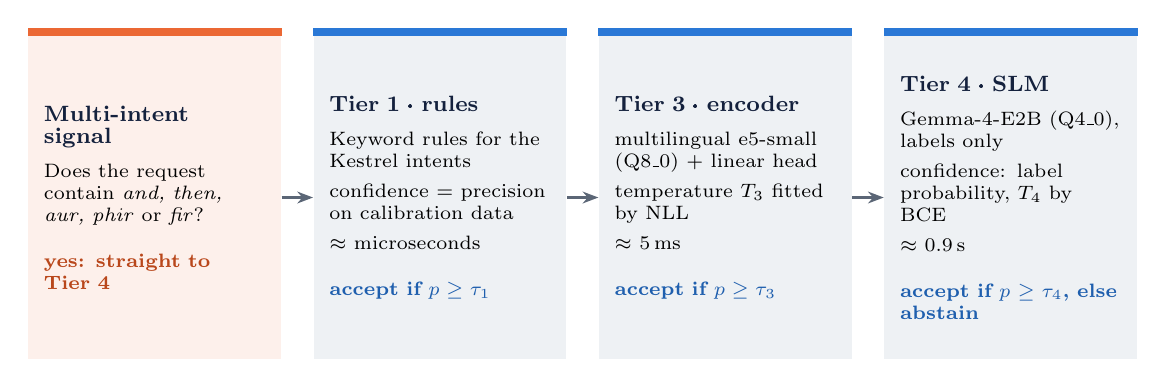
\begin{tikzpicture}[
      box/.style={fill=panel, text width=28.1mm, minimum height=41mm, inner sep=2mm, align=left,
                  font=\scriptsize, execute at begin node={\hyphenpenalty=10000\exhyphenpenalty=10000},
                  anchor=north west},
      arr/.style={-{Stealth[length=2mm]}, thick, muted}]
    \node[box, fill=warm!10] (s) at (0,0)
      {{\footnotesize\bfseries\color{ink}Multi-intent\\signal}\\[1.5mm]
       Does the request contain \emph{and, then, aur, phir} or \emph{fir}?\\[3mm]
       {\color{warmdark}\bfseries yes: straight to Tier~4}};
    \node[box] (t1) at ($(s.north east)+(4mm,0)$)
      {{\footnotesize\bfseries\color{ink}Tier 1 · rules}\\[1.5mm]
       Keyword rules for the Kestrel intents\\[1mm]
       confidence = precision on calibration data\\[1mm]
       $\approx$ microseconds\\[3mm]
       {\color{accentdark}\bfseries accept if $p\ge\tau_1$}};
    \node[box] (t3) at ($(t1.north east)+(4mm,0)$)
      {{\footnotesize\bfseries\color{ink}Tier 3 · encoder}\\[1.5mm]
       multilingual e5-small (Q8\_0) + linear head\\[1mm]
       temperature $T_3$ fitted by NLL\\[1mm]
       $\approx$ 5\ms\\[3mm]
       {\color{accentdark}\bfseries accept if $p\ge\tau_3$}};
    \node[box] (t4) at ($(t3.north east)+(4mm,0)$)
      {{\footnotesize\bfseries\color{ink}Tier 4 · SLM}\\[1.5mm]
       Gemma-4-E2B (Q4\_0), labels only\\[1mm]
       confidence: label probability, $T_4$ by BCE\\[1mm]
       $\approx$ 0.9\,s\\[3mm]
       {\color{accentdark}\bfseries accept if $p\ge\tau_4$, else abstain}};
    \fill[warm] (s.north west) rectangle ([yshift=1mm]s.north east);
    \foreach \t in {t1, t3, t4} {\fill[accent] (\t.north west) rectangle ([yshift=1mm]\t.north east);}
    \draw[arr] (s.east) -- (t1.west);
    \draw[arr] (t1.east) -- (t3.west);
    \draw[arr] (t3.east) -- (t4.west);
  \end{tikzpicture}
  \par\vspace{5mm}
  \begin{minipage}[t]{0.48\textwidth}\color{ink}No tier confident $\to$ abstain: ask the user to clarify, or
    refuse.\end{minipage}\hfill
  \begin{minipage}[t]{0.48\textwidth}\color{ink}Every $\tau$ and $T$ comes from calibration and validation data,
    frozen before test.\end{minipage}
  \slidefoot{On CLINC150 the cascade is Tier~3 $\to$ Tier~4: the Kestrel rules cannot answer with its labels.}
\end{frame}

% 4 ---------------------------------------------------------------------------------------------------------
\begin{frame}{What the closest prior work measures}{The gap}
  \vspace{2mm}
  \resizebox{\textwidth}{!}{%
  \begin{tabular}{@{}llcllc@{}}
    \toprule
    Work & What is cascaded & Calibrated & Cost measured & Rule tier & Code-mixed \\
    \midrule
    C3 (Lu 2024) & encoders or LLMs, by size & yes & FLOPs & no & no \\
    CascadeBERT (Li 2021) & BERTs, by depth & yes & FLOPs & no & no \\
    CAUC (Zhang 2026) & 2--7 models, same labels & yes & parameters, GFLOPs & no & no \\
    Arora 2024 & encoder $\to$ cloud LLM & no & API latency & no & no \\
    Chaganti 2026 & NER encoders, by size & yes & latency on device & no & no \\
    Sadhu 2026 & router $\to$ solver / SLM & n/a & latency, energy (Pi) & yes & no \\
    \rowcolor{highlight}\textbf{This work} & \textbf{rules $\to$ encoder $\to$ SLM} & \textbf{yes} &
      \textbf{latency, RAM (laptop)} & \textbf{yes} & \textbf{Hinglish} \\
    \bottomrule
  \end{tabular}}
  \par\vspace{6mm}
  {\color{ink}\large No paper in our search matches every column, but each column has close prior work.
  So this is an evaluation, not a new method.\par}
  \slidefoot{53 references checked against primary sources, none unverified.}
\end{frame}

% 5 ---------------------------------------------------------------------------------------------------------
\begin{frame}{Pre-registered hypotheses}{Research questions}
  \vspace{1mm}
  {\footnotesize
  \begin{tabular}{@{}p{31mm}p{84mm}p{18mm}@{}}
    \toprule
    Question & Hypothesis & Data \\
    \midrule
    \rowcolor{highlight}\textbf{RQ1 · H1 (primary)} &
      \textbf{Cascade R3 within $\delta=\kv{delta}$ of always-SLM R0 in accuracy, and faster} & \textbf{CLINC150} \\
    RQ1 · H1b & R3 more accurate than random escalation at the same cost & both \\
    RQ1 · H1c & R3 within $\delta$ of the encoder alone (R1) & both \\
    RQ2 · H2 & Calibration lowers selective risk at 80\% coverage & both \\
    RQ3 · H3 & Adding the encoder to rules + SLM: accuracy within $\delta$, lower cost & Intents-v0 \\
    RQ5 · H5 & Replay forgets less than naive updates of the head & CLINC150 \\
    RQ7 · H7a, H7b & Hinglish: R3 within $\delta$ of R0; higher calibration error than English & Intents-v0 \\
    RQ4, RQ6 & H4 personalization, H6 quantization: pending the dataset review & --- \\
    \bottomrule
  \end{tabular}}
  \par\vspace{2.5mm}
  {\color{muted}\small H1 is tested alone. The 13 secondary members are adjusted together by Holm's method.\par}
\end{frame}

% 6 ---------------------------------------------------------------------------------------------------------
\begin{frame}{How it was tested}{Method}
  \vspace{2mm}
  \card{0.318\textwidth}{33mm}{\head{Frozen before test}\scriptsize
    \pt{Pre-registration frozen as a git tag}
    \pt{$\delta=\kv{delta}$ from a 5-seed pilot on validation}
    \pt{Thresholds and temperatures from calibration and validation only}
    \pt{Holm across 13 secondary hypotheses}}\hfill
  \card{0.318\textwidth}{33mm}{\head{Fair baselines}\scriptsize
    \pt{R0: always the SLM, tuned abstention threshold}
    \pt{R1: the encoder alone, tuned the same way}
    \pt{R-rand: random escalation at R3's rates, same cost}
    \pt{Same models, prompts, grammar and threads}}\hfill
  \card{0.318\textwidth}{33mm}{\head{Measured on the laptop}\scriptsize
    \pt{Ryzen 5 5500U, 6 cores pinned, turbo off}
    \pt{Median of 5 timed repetitions after warm-up}
    \pt{5 invalidation rules; every test run valid first time}
    \pt{Peak RSS (VmHWM), models loaded without mmap}}
  \par\vspace{3mm}
  {\color{ink}\footnotesize CLINC150 test: \kv{clinc.n} requests, 1\,000 out of scope · Kestrel-Intents-v0 test:
  \kv{intents.n} synthetic requests, English + Hinglish\par}
  \slidefoot{Paired bootstrap, 10\,000 resamples; Intents-v0 resamples its \kv{intents.clusters} template families.}
\end{frame}

% 7 ---------------------------------------------------------------------------------------------------------
{\setbeamercolor{background canvas}{bg=ink}
 \setbeamercolor{normal text}{fg=paper}
 \setbeamercolor{frametitle}{fg=paper}
 \setbeamercolor{framesubtitle}{fg=onink}
\begin{frame}{Supported: as accurate as always-SLM, and faster}{Primary hypothesis H1 · CLINC150 test}
  \vspace{7mm}
  \begin{minipage}[t]{0.47\textwidth}
    \barred{accent}{\bignum[paper]{\kv{clinc.h1.dacc}}\vspace{1mm}
      {\color{onink}accuracy, R3 $-$ R0 · 95\% CI \kv{clinc.h1.dacc.ci}}}
  \end{minipage}\hfill
  \begin{minipage}[t]{0.47\textwidth}
    \barred{warm}{\bignum[paper]{\kv{clinc.h1.dlat}\ms}\vspace{1mm}
      {\color{onink}mean latency per request · 95\% CI \kv{clinc.h1.dlat.ci}}}
  \end{minipage}
  \par\vspace{9mm}
  {\color{paper}\large On \kv{clinc.n} requests: R3 \kv{clinc.r3.acc} vs tuned R0 \kv{clinc.r0.acc} accuracy;
  \kv{clinc.r3.tfour} reached the SLM, which answered \kv{clinc.r3.tfourans}.\par}
  \slidefoot[onink]{Margin $\delta=\kv{delta}$ · dropping the 14 duplicated test items leaves the CI unchanged.}
\end{frame}}

% 8 ---------------------------------------------------------------------------------------------------------
\begin{frame}{On CLINC150 the encoder alone was better still}{RQ1 · accuracy against latency}
  \vspace{2mm}
  \begin{minipage}[t]{0.63\textwidth}
    \vspace{0pt}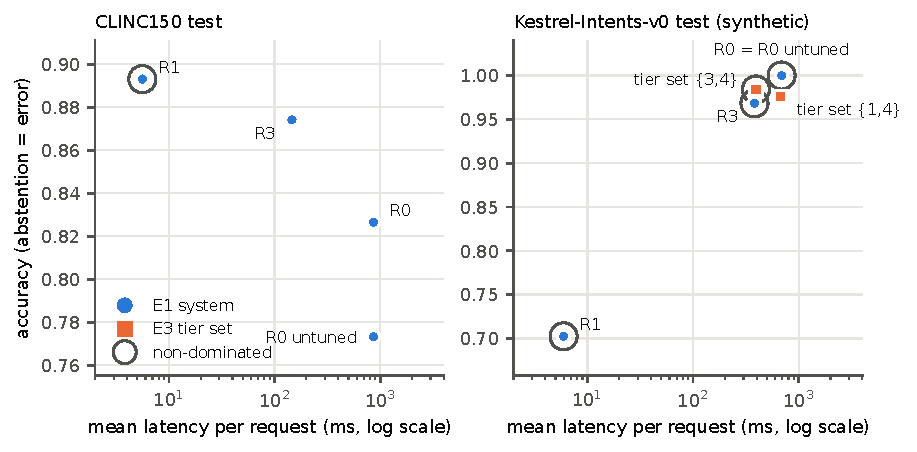
\includegraphics[width=\linewidth]{frontier.pdf}
  \end{minipage}\hfill
  \begin{minipage}[t]{0.34\textwidth}
    \vspace{0pt}\footnotesize
    \barred{accent}{\head{CLINC150}R1 \kv{clinc.r1.acc} at \kv{clinc.r1.mean}\ms\ beats R3 \kv{clinc.r3.acc} at
      \kv{clinc.r3.mean}\ms: more accurate and faster}\par\vspace{4mm}
    \barred{accent}{\head{Intents-v0}R0 is perfect (\kv{intents.r0.acc} at \kv{intents.r0.mean}\ms); R3
      \kv{intents.r3.acc} at \kv{intents.r3.mean}\ms; R1 only \kv{intents.r1.acc}}\par\vspace{4mm}
    \barred{warm}{\head{Memory}The cascade saves time, not RAM: \kv{clinc.r3.rss} vs \kv{clinc.r0.rss}~MiB peak}
  \end{minipage}
  \slidefoot{Ringed points are not dominated · H1c on CLINC150 inconclusive (Holm $p$ \kv{fam.H1c-CLINC150.holm}).}
\end{frame}

% 9 ---------------------------------------------------------------------------------------------------------
\begin{frame}{Calibration lowered risk on CLINC150 only}{RQ2 · calibration (E2)}
  \vspace{2mm}
  \begin{minipage}[t]{0.63\textwidth}
    \vspace{0pt}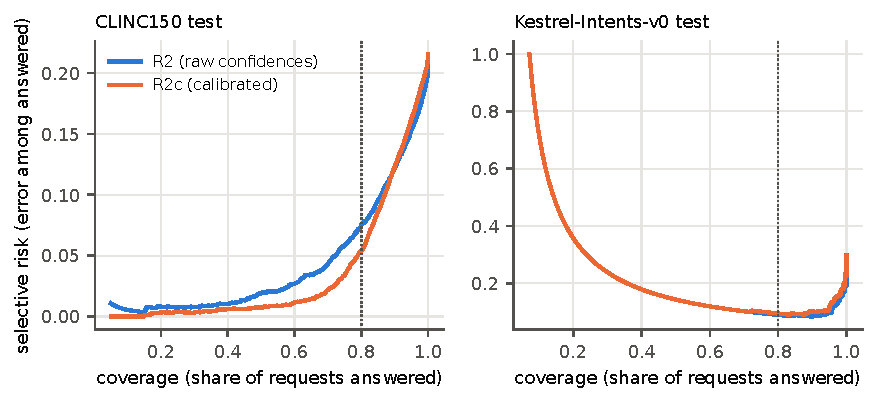
\includegraphics[width=\linewidth]{riskcov.pdf}
  \end{minipage}\hfill
  \begin{minipage}[t]{0.34\textwidth}
    \vspace{0pt}\footnotesize
    \barred{accent}{\head{CLINC150 · supported}Risk at 80\% coverage \kv{clinc.risk.rtwo} $\to$
      \kv{clinc.risk.rtwoc}; $\Delta$ \kv{clinc.risk.diff} \kv{clinc.risk.diff.ci}\par\vspace{1mm}
      Encoder ECE \kv{clinc.tthree.ece.before} $\to$ \kv{clinc.tthree.ece.after}}\par\vspace{4mm}
    \barred{warm}{\head{Intents-v0 · inconclusive}\kv{intents.risk.rtwo} $\to$ \kv{intents.risk.rtwoc};
      $\Delta$ \kv{intents.risk.diff} \kv{intents.risk.diff.ci}}\par\vspace{4mm}
    \barred{muted}{\head{Why it helps}Per-tier risk barely moved; the gain is making tiers comparable under one
      threshold}
  \end{minipage}
  \slidefoot{R2: raw confidences · R2c: temperature-scaled · one shared threshold.}
\end{frame}

% 10 --------------------------------------------------------------------------------------------------------
\begin{frame}{The encoder tier pays; replay stops forgetting}{RQ3 and RQ5 · tiers and forgetting}
  \vspace{2mm}
  \card{0.485\textwidth}{44mm}{\kicker{E3 tier ablation · Intents-v0 · H3 supported}
    \bignum{\kv{intents.hthree.dcost}\ms}\vspace{1mm}
    mean cost of adding the encoder to rules + SLM · CI \kv{intents.hthree.dcost.ci}\par\vspace{2mm}
    {\footnotesize Accuracy $\Delta$ \kv{intents.hthree.dacc} \kv{intents.hthree.dacc.ci}, within $\delta$\par
    \vspace{1mm}Rules cost accuracy: \{1,4\} \kv{intents.set14.acc} vs \{4\} \kv{intents.set4.acc}\par}}\hfill
  \card[warm]{0.485\textwidth}{44mm}{\kicker{E5 head updates · CLINC150, 15 runs · H5 supported}
    \bignum{\kv{e5.replay.acc}}\vspace{1mm}
    average accuracy with replay, vs \kv{e5.naive.acc} naive (joint \kv{e5.joint.acc})\par\vspace{2mm}
    {\footnotesize Forgetting: naive \kv{e5.naive.forget}, replay \kv{e5.replay.forget}; EWC $\approx$ naive
    (\kv{e5.ewc.forget})\par\vspace{1mm}
    Price: a buffer of half of each old class's training items, as embeddings (\kv{e5.replay.buffer}~MB)\par}}
  \slidefoot{Tier 2 (distilled model) was not built · E5: 10 domains in 5 stages, 3 orders $\times$ 5 seeds.}
\end{frame}

% 11 --------------------------------------------------------------------------------------------------------
\begin{frame}{Every pre-registered test, with its outcome}{All hypotheses}
  \vspace{2mm}
  \begin{minipage}[t]{0.19\textwidth}\statnum{1 of 1}{primary supported}\end{minipage}\hfill
  \begin{minipage}[t]{0.19\textwidth}\statnum{\kv{fam.supported} of 13}{secondary supported}\end{minipage}\hfill
  \begin{minipage}[t]{0.19\textwidth}\statnum{5}{inconclusive}\end{minipage}\hfill
  \begin{minipage}[t]{0.19\textwidth}\statnum{0}{not supported}\end{minipage}\hfill
  \begin{minipage}[t]{0.19\textwidth}\statnum{2}{pending (E4, E6)}\end{minipage}
  \par\vspace{4mm}
  \begin{minipage}[t]{0.485\textwidth}
    \resizebox{\linewidth}{!}{%
    \begin{tabular}{@{}lll@{}}
      \toprule
      Hypothesis & Holm $p$ & Outcome \\
      \midrule
      H1 CLINC150 (primary) & \kv{clinc.h1.p} (alone) & \kv{clinc.h1.outcome} \\
      H1b CLINC150 & \kv{fam.H1b-CLINC150.holm} & \kv{fam.H1b-CLINC150.outcome} \\
      H1b Intents-v0 & \kv{fam.H1b-Intents-v0.holm} & \kv{fam.H1b-Intents-v0.outcome} \\
      H1c CLINC150 & \kv{fam.H1c-CLINC150.holm} & \kv{fam.H1c-CLINC150.outcome} \\
      H1c Intents-v0 & \kv{fam.H1c-Intents-v0.holm} & \kv{fam.H1c-Intents-v0.outcome} \\
      H1 Intents-v0 & \kv{fam.H1-Intents-v0.holm} & \kv{fam.H1-Intents-v0.outcome} \\
      H2 CLINC150 & \kv{fam.H2-CLINC150.holm} & \kv{fam.H2-CLINC150.outcome} \\
      \bottomrule
    \end{tabular}}
  \end{minipage}\hfill
  \begin{minipage}[t]{0.485\textwidth}
    \resizebox{\linewidth}{!}{%
    \begin{tabular}{@{}lll@{}}
      \toprule
      Hypothesis & Holm $p$ & Outcome \\
      \midrule
      H2 Intents-v0 & \kv{fam.H2-Intents-v0.holm} & \kv{fam.H2-Intents-v0.outcome} \\
      H3 encoder tier & \kv{fam.H3.holm} & \kv{fam.H3.outcome} \\
      H5 replay vs naive & \kv{fam.H5.holm} & \kv{fam.H5.outcome} \\
      H7a Hinglish accuracy & \kv{fam.H7a.holm} & \kv{fam.H7a.outcome} \\
      H7b Hinglish ECE & \kv{fam.H7b.holm} & \kv{fam.H7b.outcome} \\
      H4 personalization & --- & \kv{fam.H4.outcome} \\
      H6 quantization & --- & \kv{fam.H6.outcome} \\
      \bottomrule
    \end{tabular}}
  \end{minipage}
  \slidefoot{H1 tested alone · Holm interim until H4, H6 run: ``supported'' is final, ``inconclusive'' may change.}
\end{frame}

% 12 --------------------------------------------------------------------------------------------------------
\begin{frame}{Why the cascade lost where it did}{Failure analysis · exploratory}
  \vspace{2mm}
  \card{0.485\textwidth}{37mm}{\kicker{CLINC150 · out-of-scope shift}
    \bignum{\kv{err.clinc.oosshare}}\vspace{1mm}
    {\small of R3's \kv{err.clinc.errors} errors are out-of-scope requests answered as in-scope\par}\vspace{2mm}
    {\scriptsize Out-of-scope share: \kv{err.clinc.oos.val} of validation, \kv{err.clinc.oos.test} of test\par
    \vspace{1mm}\kv{err.clinc.band} out-of-scope test requests fall between R3's \kv{err.clinc.tau.rthree} and R1's
    \kv{err.clinc.tau.rone} thresholds\par}}\hfill
  \card[warm]{0.485\textwidth}{37mm}{\kicker{Intents-v0 · multi-intent gap}
    \bignum{\kv{err.intents.compound} of \kv{err.intents.errors}}\vspace{1mm}
    {\small of R3's errors are two-part requests joined by ``also'' or ``, now''\par}\vspace{2mm}
    {\scriptsize The signal knows only \emph{and, then, aur, phir, fir}; all \kv{err.intents.valcompounds}
    validation compounds had one\par}}
  \par\vspace{4mm}
  {\color{ink}\small Fixes (Tier-3 reject band, out-of-scope detector, wider signal) need a new pre-registered
  version.\par}
  \slidefoot{ECE \kv{clinc.tthree.ece.after} after scaling covers in-scope items only; calibration on out-of-scope
  requests is untested.}
\end{frame}

% 13 --------------------------------------------------------------------------------------------------------
\newcommand{\limitem}[2]{\barred{accent}{{\footnotesize\bfseries\color{ink}#1\par}\vspace{0.5mm}
  {\scriptsize #2\par}}\par\vspace{2.5mm}}
\begin{frame}{What these results do not show}{Limitations}
  \vspace{2mm}
  \begin{minipage}[t]{0.48\textwidth}
    \limitem{One machine}{one CPU, one SLM, one encoder; turbo off}
    \limitem{Synthetic data}{Intents-v0 drafted with AI help; $\kappa$ not yet measured}
    \limitem{Small Hinglish set}{126 requests per language; wide intervals}
    \limitem{E4, E6 pending}{personalization and quantization wait on the dataset review}
    \limitem{Warm process only}{latency excludes model loading; one warm, single-user process}
  \end{minipage}\hfill
  \begin{minipage}[t]{0.48\textwidth}
    \limitem{Reproduced here only}{byte-identical reruns here; a second machine next week}
    \limitem{$\delta$ before SESOI}{margin frozen before the smallest effect of interest was confirmed}
    \limitem{No energy}{the only counter (RAPL) is root-only here}
    \limitem{Privacy tested}{\kv{priv.pass} of \kv{priv.total} checks pass; not a formal guarantee}
  \end{minipage}
  \slidefoot{Full list: experiments/LIMITATIONS.md and the paper's threats to validity.}
\end{frame}

% 14 --------------------------------------------------------------------------------------------------------
\begin{frame}{What the evidence supports, and what is next}{Conclusion}
  \vspace{2mm}
  \card{0.575\textwidth}{46mm}{\head{Answers}\footnotesize
    \textbf{RQ1} · yes against the SLM on CLINC150 (\kv{clinc.h1.dacc}, \kv{clinc.h1.dlat}\ms); no against the
    encoder alone\par\vspace{1.5mm}
    \textbf{RQ2} · calibration lowers risk on CLINC150; not replicated on synthetic data\par\vspace{1.5mm}
    \textbf{RQ3} · the encoder tier changes mean cost by \kv{intents.hthree.dcost}\ms, accuracy within $\delta$
    \par\vspace{1.5mm}
    \textbf{RQ5} · replay prevents forgetting; EWC does not\par\vspace{1.5mm}
    \textbf{RQ7} · Hinglish: inconclusive}\hfill
  \card[warm]{0.395\textwidth}{46mm}{\head{Next}\footnotesize
    \begin{enumerate}\setlength{\itemsep}{1mm}
      \item Review the Tasks and Personas datasets; freeze amendment v1.1
      \item Run E4 and E6; final Holm family
      \item Reproduce on a second machine (Mac)
      \item Second annotator ($\kappa$); confirm the smallest effect of interest
    \end{enumerate}}
  \slidefoot{Paper draft, code, logs and the one-command reproduction (experiments/repro.py) are in the repository.}
\end{frame}

\end{document}
